\section{Architecture}
\subsection{Server}
The server has two communications parts and one storage backend. The first communications part is responsible for talking the the aggregator placed in the users home, it will poll data from this device and place them in a database. The second part is responsible for talking with users Android devices and feeding them data from their own aggregator box and other usage data such as friends data and general statistics. The storage backends is responsible for keeping data updated and available.

\begin{figure}[H]
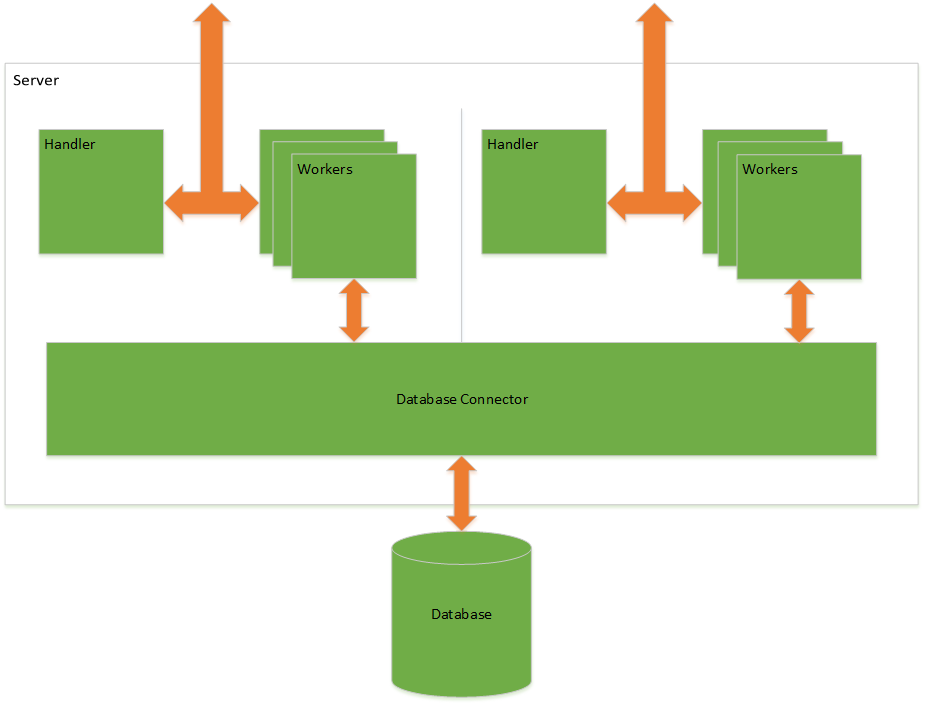
\includegraphics[width=\textwidth]{ch/projectPlan/fig/server.png}
\caption{Server}
\end{figure}

\subsection{Android Device}
The application running on the Android device will be responsible for handling connections to external services like Google Drive and Facebook as well as fetching data from the server.

\begin{figure}[H]
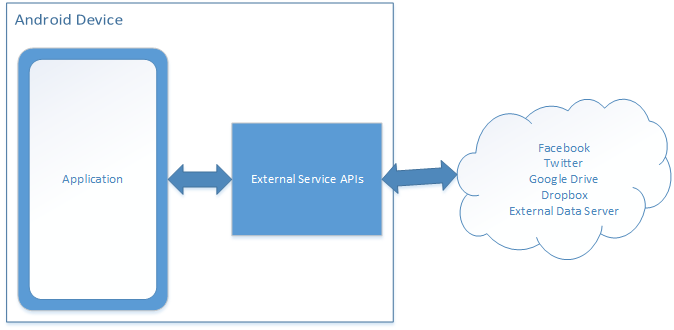
\includegraphics[width=\textwidth]{ch/projectPlan/fig/androidDevice.png}
\caption{Android device}
\end{figure}

\subsection{Home Data Aggregator}
This device will collect data from sources in the users home. The reason for this external box as opposed to using the users phone to collect data, is with this solution we can fetch data at regular intervals throughout the whole day with no need for the users to be home. The device will pass data along to the external server at request from the server.

\begin{figure}[H]
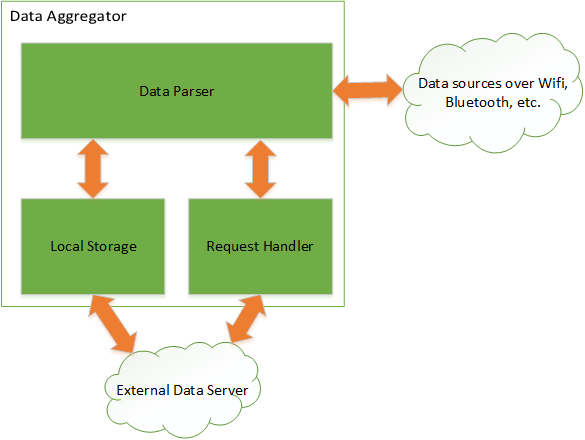
\includegraphics[width=\textwidth]{ch/projectPlan/fig/home.png}
\caption{Home data aggregator}
\end{figure}
